\documentclass[11pt]{report}
\usepackage{graphicx}
\usepackage{amsmath}
\usepackage{amsthm}
\usepackage[spanish]{babel}
\usepackage{rotating,stackengine,scalerel}
\usepackage{blindtext}
\usepackage[a4paper, total={6in, 8in}]{geometry}
\newcommand\wye{\scalerel*{\stackengine{-1pt}{
      \rotatebox[origin=c]{30}{\rule{10pt}{.9pt}}\kern-1pt
      \rotatebox[origin=c]{-30}{\rule{10pt}{1.3pt}}}{
      \rule{.9pt}{10pt}}{O}{c}{F}{F}{S}}{\Delta}}

\newtheorem{example}{Ejemplo}[section]

\title{Máquinas y Comandos Eléctricos}
\author{Joaquín Gómez --- 5to ``A''}
\date{2025}

\begin{document}
\maketitle

\chapter{Autotransformadores}
Los autotransformadores poseen una parte del devanado en común, que corresponde
tanto al
primario como al secundario.
El principio de funcionamiento es el mismo que el del transformador común,
entonces la relación de
transformación entre las tensiones, las intensidades de corriente y el número
de vueltas se mantienen.

Las corrientes primarias y secundarias están en oposición y la corriente total
que circula por las espiras
en común es igual a la diferencia de la corriente del devanado de baja tensión
y el devanado de alta tensión
\begin{equation}
  I_c = I_{AT} - I_{BT} \quad \textnormal{si } V_{AT} > V_{BT}
\end{equation}
Para que un autotransformador funcione adecuadamente, los devanados deben tener
el mismo sentido de bobinado.

\section{Autotransformadores Reductores}
Si se aplica una tensión alterna entre los puntos A y B, y se mide la tensión
de salida entre los puntos C y D,
se dice que el autotransformador es un reductor de tensión

\begin{figure}[h]
  \begin{center}
    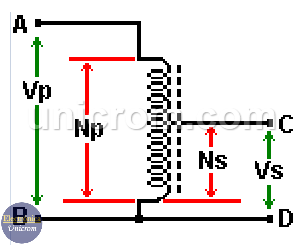
\includegraphics[width=200px]{autotransformador-reductor.png}
  \end{center}
  \caption{Autotransformador reductor}
\end{figure}

En este caso, la relación de vueltas del autotransformador es:
\begin{equation}
  \frac{N_s}{N_p} < 1
\end{equation}

\section{Autotransformadores elevadores}
Si se aplica una tensión de alimentación alterna entre los puntos A y B, y se
mide la tensión de salida entre los puntos C y D, se dice que el
autotransformador es elevador de tensión.

\begin{figure}[h]
  \begin{center}
    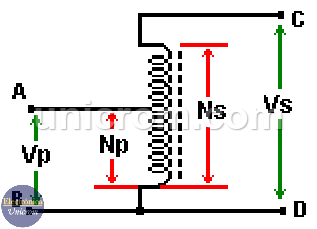
\includegraphics[width=200px]{autotransformador-elevador.png}
  \end{center}
  \caption{Autotransformador elevador}
\end{figure}

En este caso, la relación de vueltas del autotransformador es:
\begin{equation}
  \frac{N_s}{N_p} > 1
\end{equation}

Los autotransformadores tienen la ventaja sobre los transformadores comunes
de un peso y costo menor. En lugar de tener un bobinado de AT de $N_1$ espiras,
se debe preveer para el bobinado de BT, con un número $N_2$ de espiras, un
número
adicional de espiras de $N_1-N_2$. También hay que tener en cuenta que el
conductor
de la sección común del bobinado debe tener una sección de alambre en función
de la
diferencia de corrientes entre AT y BT, o sea, $I_2-I_1$.

Otra ventaja es la de no necesitar aislamiento entre los bobinados primario y
secundario.
Sin embargo, esto trae como desventaja que el bobinado primario no es
independiente del
secundario. Esto causa peligro para una persona, pues, entre tierra y el hilo
común del
secundario y el primario existe la tensión del primario (Ver figura 1).

\begin{example}
  Se requiere un autotransformador para aumentar un voltaje de $220V$ a
  $250V$.
  El número total de espiras que tiene el devanado principal es de
  $2000$. Determine
  la posición del punto de toma primario, la corriente primaria y
  secundaria cuando
  la salida tiene una potencia de $10{kVA}$. Y la economía de cobre
  ahorrada\footnote{La
    relación $n$ se define como la relación entre el voltaje más bajo y el
    voltaje más alto,
    entonces se puede demostrar que el ahorro de cobre es: $n\cdot100\%$}.

  Tenemos que la relación ideal de vueltas debe ser
  \begin{equation}
    \frac{V_1}{V_2} < 1
  \end{equation}
  ya que el transformador es elevador. De forma que
  \begin{equation}
    \frac{N_1}{N_2} < 1
  \end{equation}
  Así, tenemos que idealmente
  \begin{equation}
    \begin{split}
      \frac{V_1}{V_2} &= \frac{N_1}{N_2} \\
      \frac{220V}{250V} &= \frac{N_1}{2000esp} \\
    \end{split}
  \end{equation}
  Por lo tanto
  \begin{equation}
    \begin{split}
      N_2 &= \frac{220 V \cdot 2000esp}{250V} \\&= 1760 esp
    \end{split}
  \end{equation}
  El porcentaje de ahorro de cobre está dado por
  \begin{equation}
    n\cdot 100\% = \frac{V_1}{V_2}\cdot 100\% = 88\%
  \end{equation}
  Como condición, tenemos que $P_1 = P_2$, así, podemos deducir que
  \begin{equation}
    \begin{split}
      V_1 I_1 &= P_1 \\
      220V I_1 &= 10000VA \\
      I_1 &\approx 45.456A
    \end{split}
  \end{equation}
  \begin{equation}
    \begin{split}
      V_2 I_2 &= P_2 \\
      250V I_2 &= 10000VA \\
      I_2 &= 40A
    \end{split}
  \end{equation}
\end{example}

\begin{example}
  En el siguiente autotransformador reductor indicar el sentido de la
  corriente ($I_c$, intensidad común) que circulará por la parte del
  arrollamiento que tienen en común $N_1$ y $N_2$. Fundamentar el sentido de
  circulación.

  Si tenemos un transformador reductor, donde $V_1 > V_2$, entonces $I_1
    < I_2$. Por la ley de Kirchoff tenemos
  \begin{equation}
    \sum_k I_s^{(k)} = \sum_k I_e^{(k)}
  \end{equation}
  es decir, la suma de las corrientes de entrada es igual a las de
  salida. En este caso, si $I_1 < I_2$ tendremos
  \begin{equation}
    I_2 = I_1 + I_C
  \end{equation}
  Como la corriente $I_1$ es la entrada, tenemos que $I_2$ y $I_c$ serán
  corrientes de salida.
  \begin{center}
    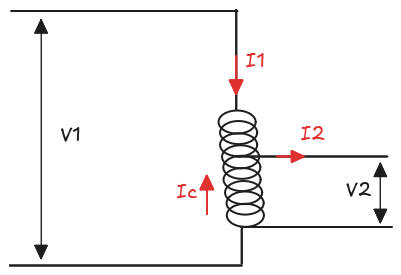
\includegraphics[width=200px]{ejemplo2.png}
  \end{center}
\end{example}

\chapter{Transformadores Trifásicos}

\section{Introducción}
La mayoría de los transformadores utilizados en la transmisión y distribución
de energía eléctrica
son trifásicos por una cuestión de costos, tamaños y transporte; pero hay
excepciones: cuando las
potencias son muy grandes, de cientos de $m\,{\textnormal{VA}}$ (mega
volt-amper), o se requiren varios transformadores
de gran potencia, e iguales. Por ejemplo, en una central con una cierta
cantidad de máquinas de gran potencia,
puede convenir utilizar bancos trifásicos armados con tres transformadores del
tipo monofásicos, e inclusive,
tener algún transformador de reserva.

Se puede decir que un transformador trifásico está constituido por tres
transformadores tipo monofásicos montados
en un núcleo magnético en común. La constitución más común es la de
\textit{tres columnas}, con los arrollamientos
primarios y secundarios alternados o concéntricos.

El estudio del transformador trifásico se puede reducir al monofásico a
condición de trabajar con los valores por fase.
En este sentido, habrá que tener en cuenta la fórmula de potencia a aplicar, en
vacío, en carga o en cortocircuito. Deberá
ser trifásica y no monofásica.

Los devanados tanto en el primario como en el secundario, pueden estar
acoplados en:

$\wye$ Estrella: $Y$ (en el bobinado de AT), $y$ (en el bobinado de BT)

$\triangle$ Triángulo: $D$ (en el bobinado de AT), $d$ (en el bobinado de BT)

$??$ Zig zag: $Z$ (en el bobinado de AT), $z$ (en el bobinado de BT)

Por convención se adopta la letra mayúscula para indicar la forma de conexión
del devanado primario y minúscula la del bobinado
secundario.

Tenemos nueve posibles formas de conexión, dadas por
\begin{equation*}
  \begin{matrix}
    Y_y & D_y & Z_y \\
    Y_d & D_d & Z_d \\
    Y_z & D_z & Z_z \\
  \end{matrix}
\end{equation*}
(Son nueve porque tenemos 3 opciones, el total es el conjunto $(Y,D,Z)\times
  (y,d,z)$)
Por ejemplo, $Y_d$ denota una conexión primaria en estrella y secundario en
triángulo.
Las denominaciones son
\begin{equation*}
  \begin{aligned}
     & Y_y = \textnormal{ Estrella-Estrella}   \\
     & Y_d = \textnormal{ Estrella-Triángulo}  \\
     & Y_z = \textnormal{ Estrella-Zigzag}     \\
     & D_y = \textnormal{ Triángulo-Estrella}  \\
     & D_d = \textnormal{ Triángulo-Triángulo} \\
     & D_z = \textnormal{ Triángulo-Zigzag}    \\
     & Z_y = \textnormal{ Zigzag-Estrella}     \\
     & Z_d = \textnormal{ Zigzag-Triángulo}    \\
     & Z_z = \textnormal{ Zigzag-Zigzag}       \\
  \end{aligned}
\end{equation*}
Siendo las primeras seis las más utilizadas.
Si algún devanado tiene neutro accesible, al símbolo correspondiente se le
señana la letra
`$o$' o `$n$'.

\begin{center}
  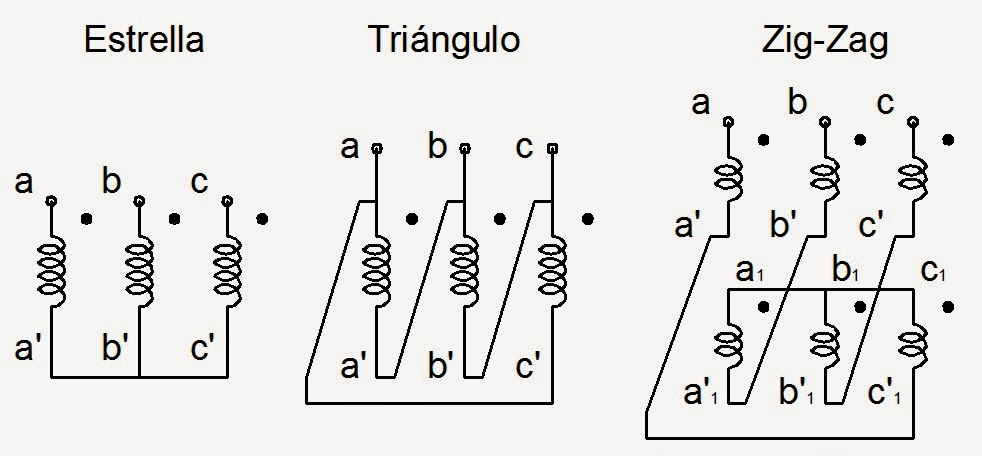
\includegraphics[width=300px]{conexiones-trafo.jpg}
\end{center}

La transformación de tensiones en los sistemas trifásicos
pueden realizarse de dos maneras distintas.

De acuerdo a la estructura del núcleo, las más empleadas son las siguientes

\subsection{Transformador con sistema magnético acoplado}
Es denominado como transformador de \textbf{tres columnas} o \textbf{núcleo
  trifásico};
tiene una asimetría en el circuito magnético, lo que origina que las tres
corrientes de excitación no sean iguales.

\begin{center}
  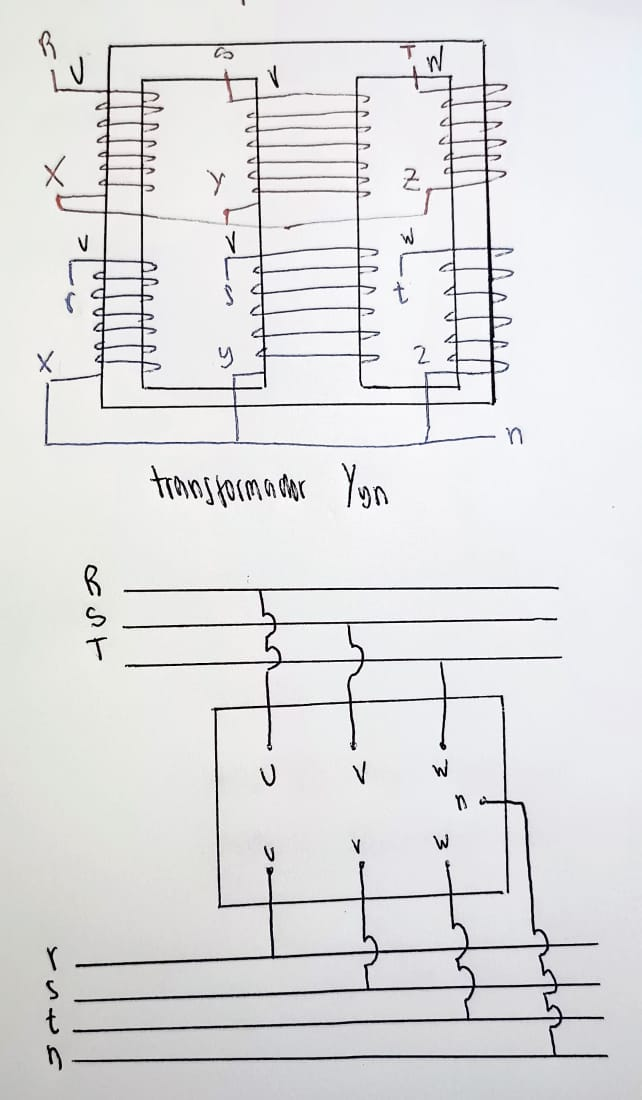
\includegraphics[width=300px]{trafo-trifasico.jpeg}
\end{center}

\subsection{Transformador con sistema magnético independiente}
Denominado también banco de transformación trifásica a base de transformadores
monofásicos o
grupo transformador trifásico. En este caso se tienen tres circuitos magnéticos
independientes,
por lo que las corrientes de excitación serán iguales

\begin{center}
  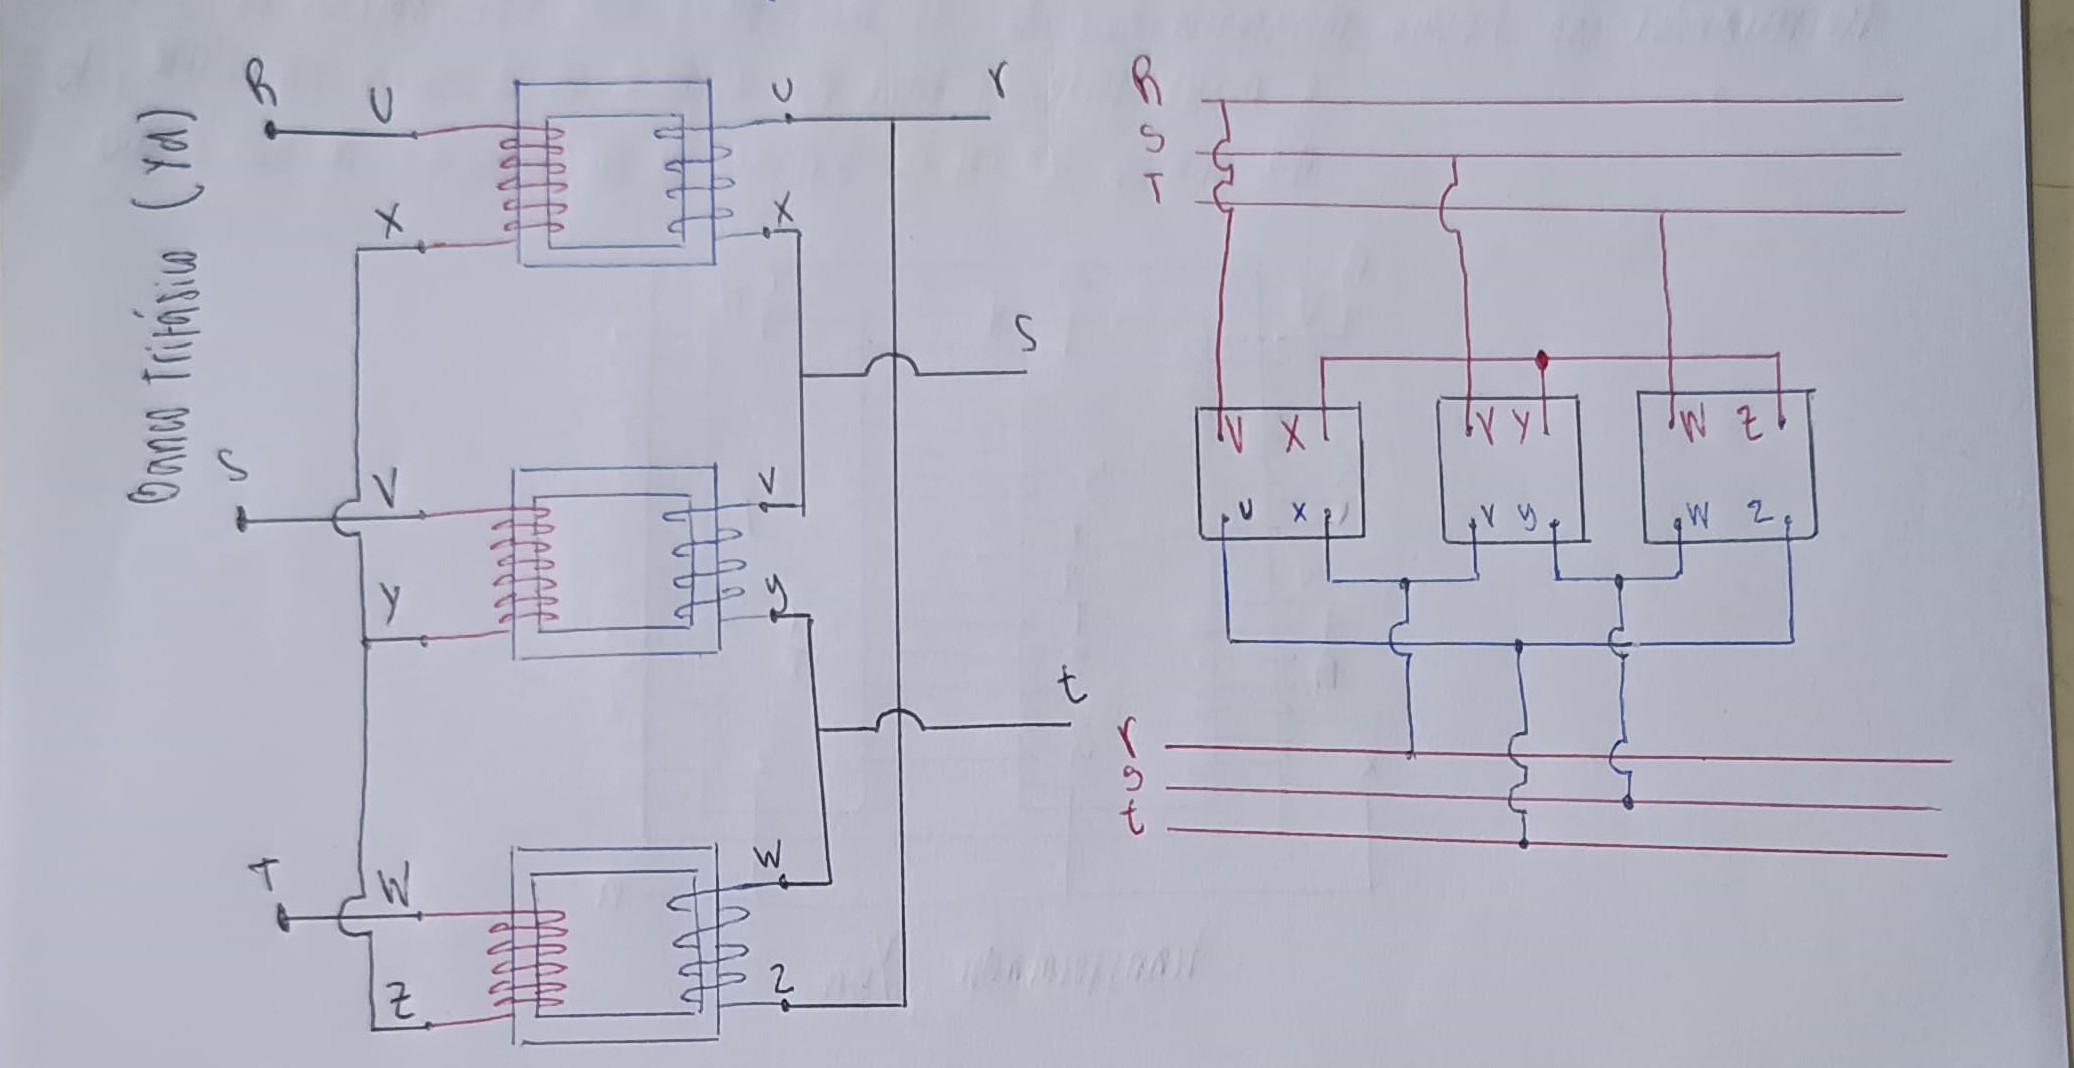
\includegraphics[width=360px]{trafo-independiente.jpeg}
\end{center}

A continuación se desarrollarán las conexiones más utilizadas de
transformadores trifásicos.

\pagebreak
\section{Conexión triángulo-triángulo ($D_d$)}
Para esta clase de trafo., las 3 fases del bobinado primario y
secundario están conectados en triángulo. Esta conexión se expresa
abreviadamente con el símbolo $D_d$.

\begin{center}
  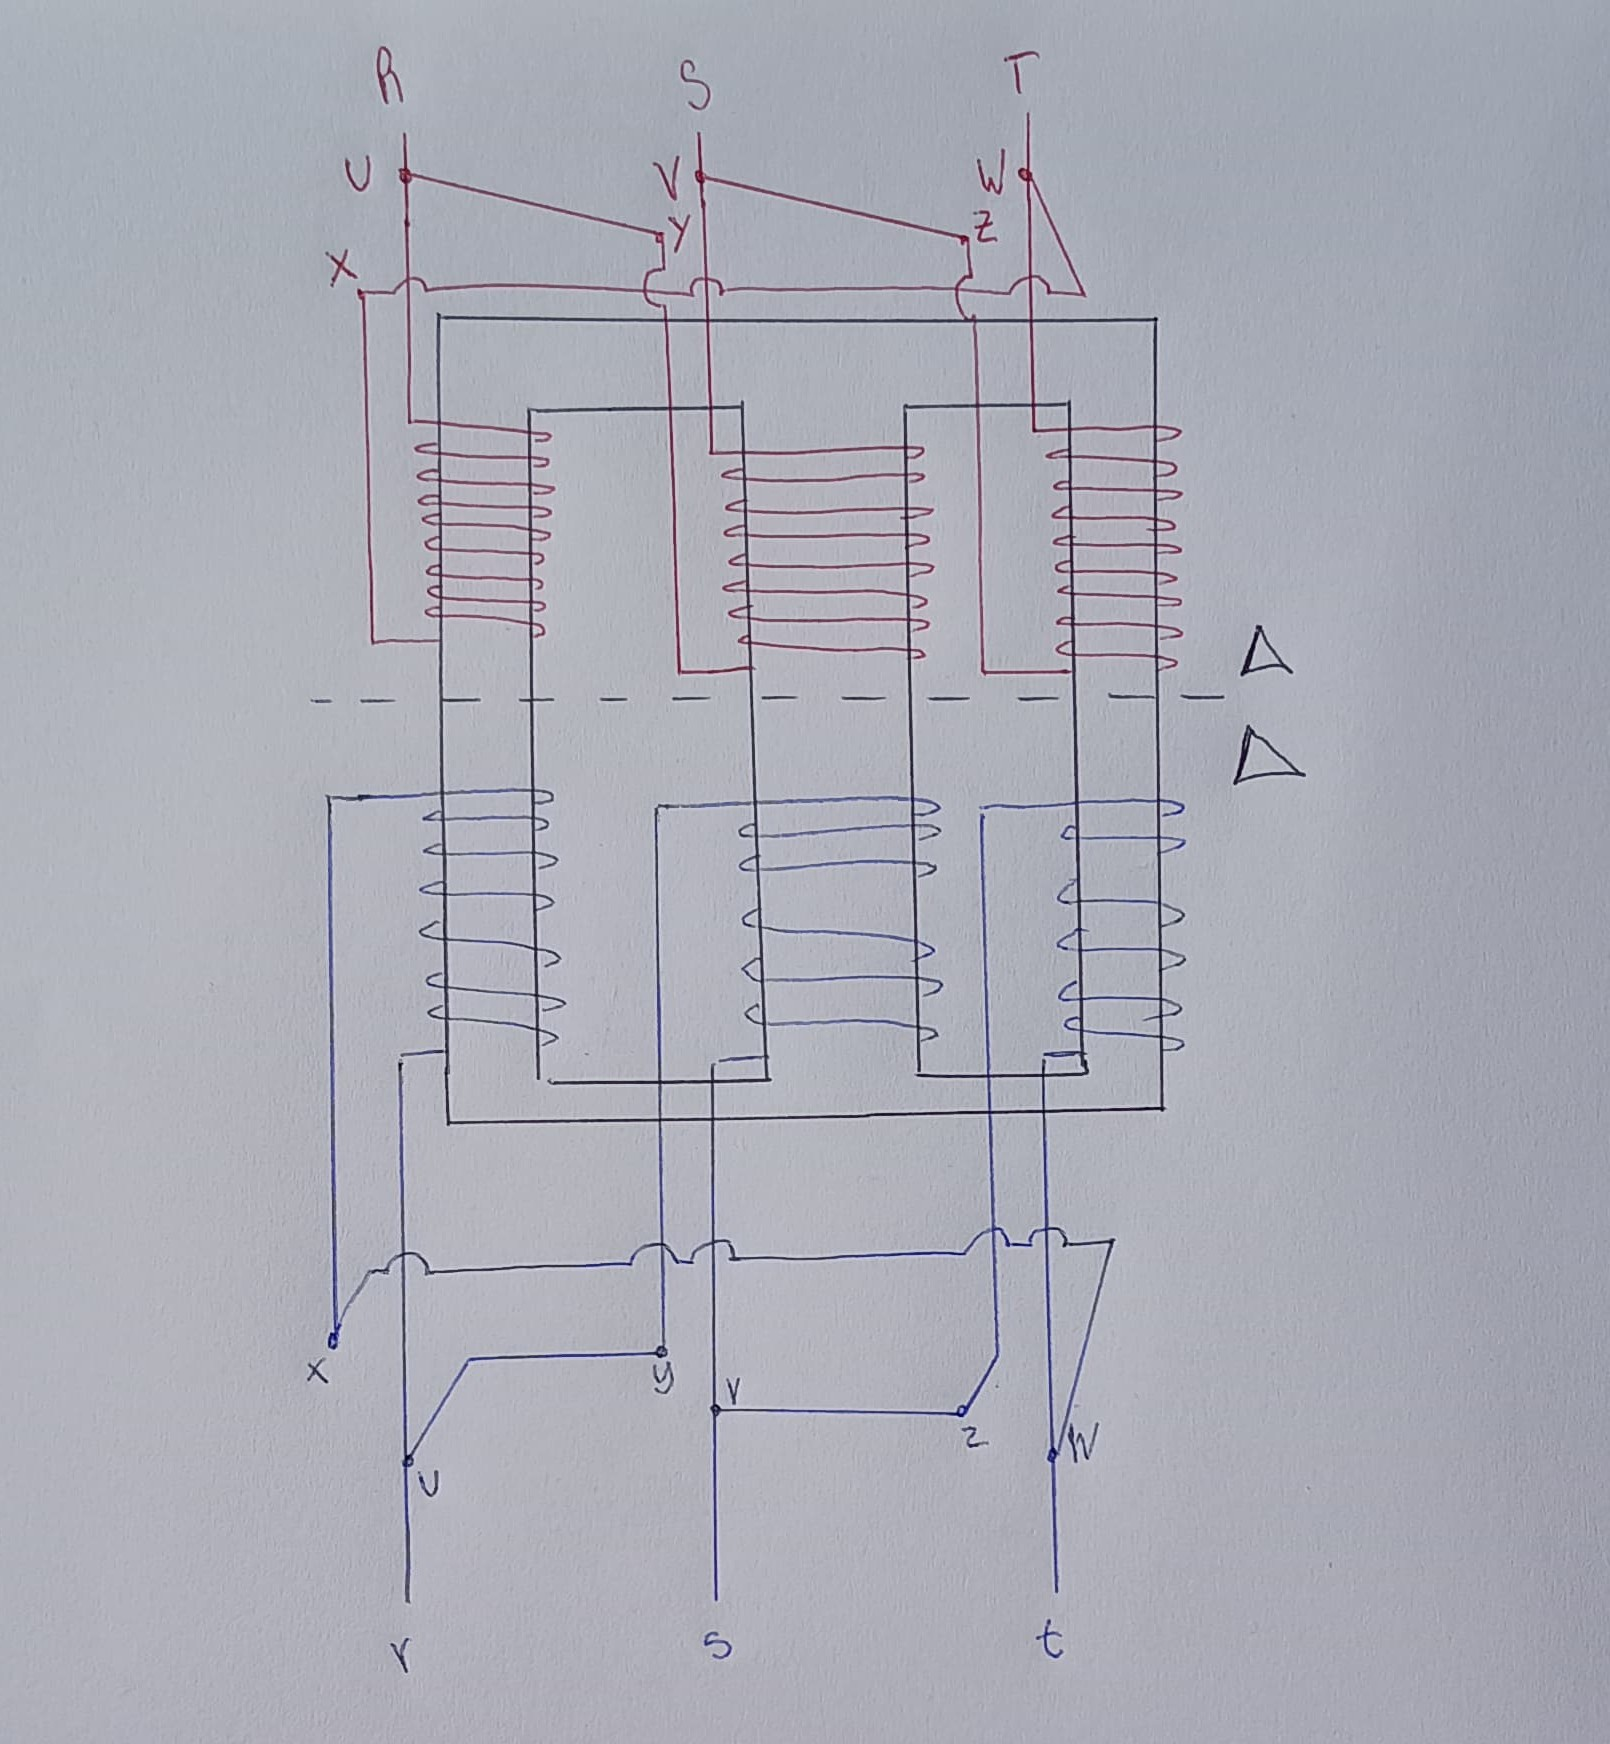
\includegraphics[width=300px]{trafo-conexion-dd.jpeg}
\end{center}
\pagebreak
\section{Conexión estrella-estrella ($Y_y$)}
En esta clase de transformador trifásico, las tres fases de ambos bobinados
están conectadas en estrella. Esta conexión se expresa con el símbolo $Y_y$.

\begin{center}
  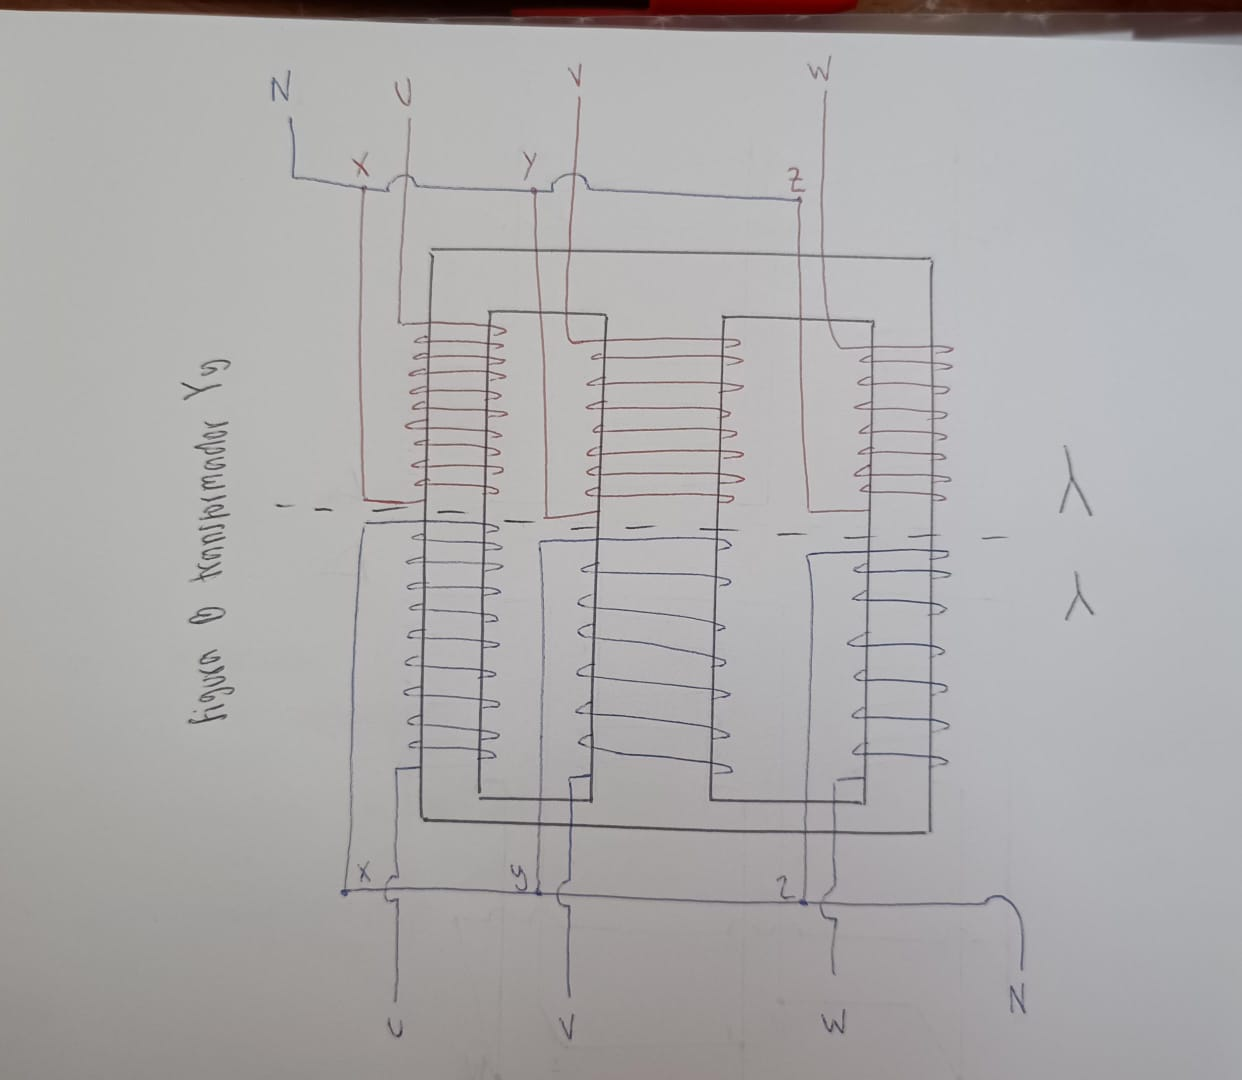
\includegraphics[width=300px]{trafo-conexion-yy.jpeg}
\end{center}

La conexión estrella se utiliza cuando la línea tiene neutro, el neutro se
emplea siempre en baja tensión, mientras que en alta tensión se uusa poco ya
que ahorrar en conductor supone en una línea de alta tensión un ahorro muy
importante, ya que generalmente las líneas de AT tienen muchos kilómetros de
largo.

\pagebreak
\section{Conexión triángulo-estrella ($D_y$)}
En esta clase de transformador trifásico las tres fases del bobinado primario
están conectadas en triángulo, mientras que las tres fases del bobinado
secundario están en estrella. Ésta conexión se expresa con el símbolo $D_y$.

\begin{center}
  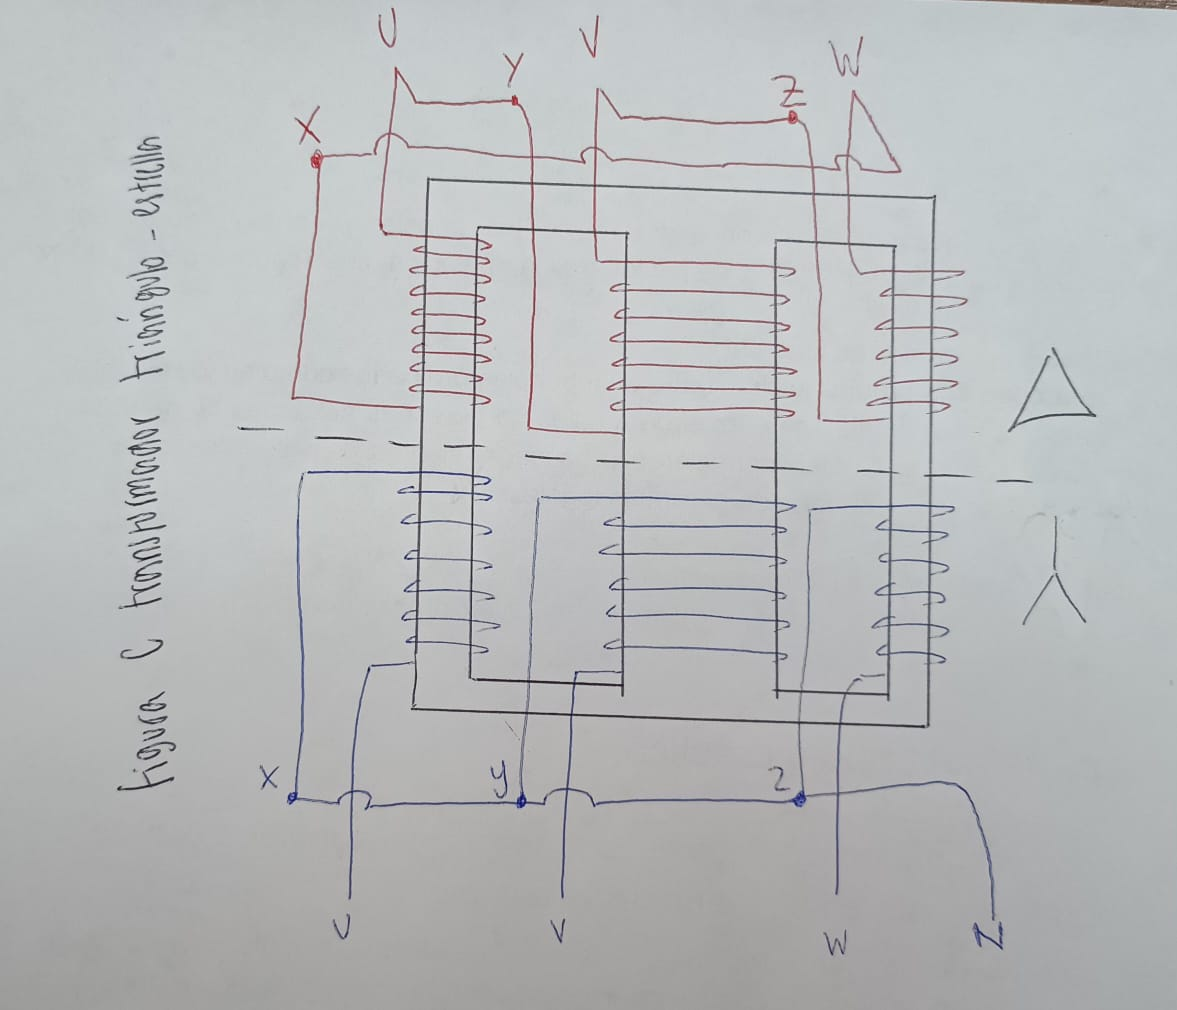
\includegraphics[width=300px]{trafo-conexion-dy.jpeg}
\end{center}
\pagebreak

\section{Conexión estrella-triángulo ($Y_d$)}
En el transformador estrella-triángulo las tres fases del bobinado primario
están conectadas en estrella, mientras que las tres fases del bobinado
secundario lo están en triángulo. Ésta conexión es expresada
abreviadamente por el símbolo $Y_d$.

\begin{center}
  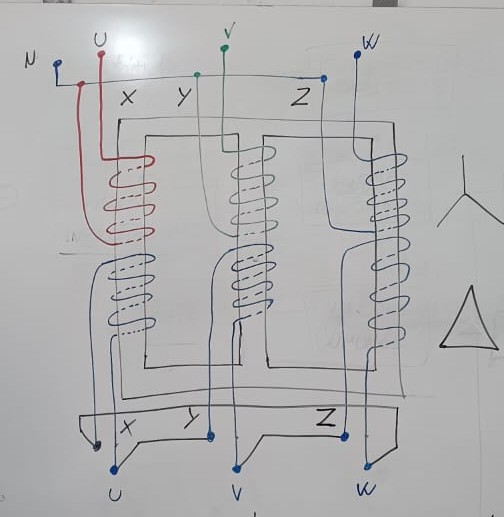
\includegraphics[width=300px]{trafo-conexion-yd.jpeg}
\end{center}

\section{Representación de las tensiones e intensidades en las conexiones más
  usuales de transformadores trifásicos}

Para tener en cuenta, en la representación de las conexiones, la relación de
transformación se aplicará de forma similar que en los transformadores
monofásicos.
\pagebreak
\begin{enumerate}
  \item $Y \triangle$ --- $Y_d$
        \begin{center}
          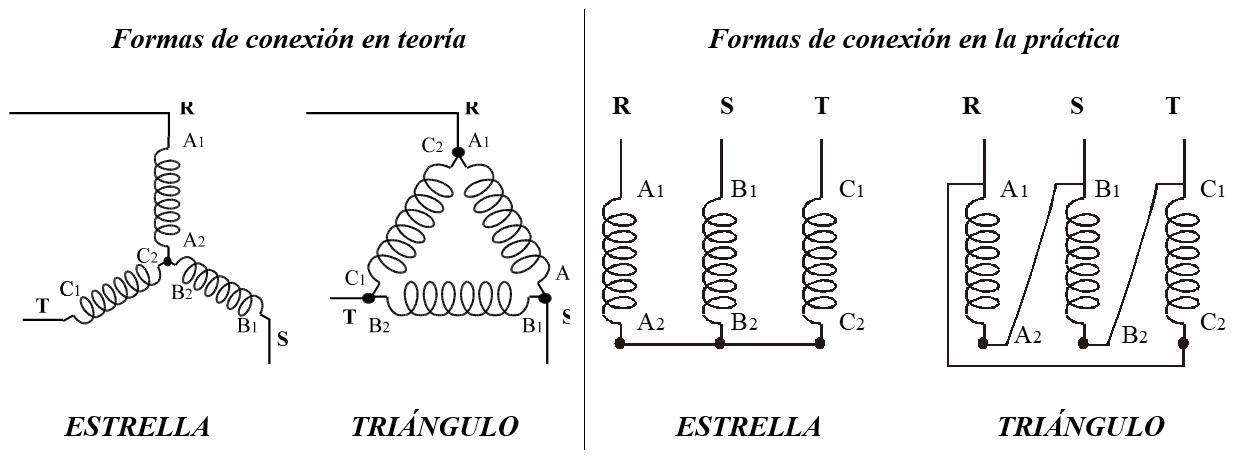
\includegraphics[width=400px]{estrella-triangulo-trafo.png}
        \end{center}
  \item $YY$ --- $Y_y$
        \begin{center}
          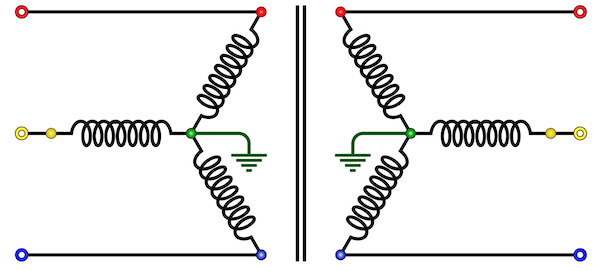
\includegraphics[width=400px]{estrella-estrella-trafo.png}
        \end{center}

  \item $\triangle Y$ --- $D_y$
        \begin{center}
          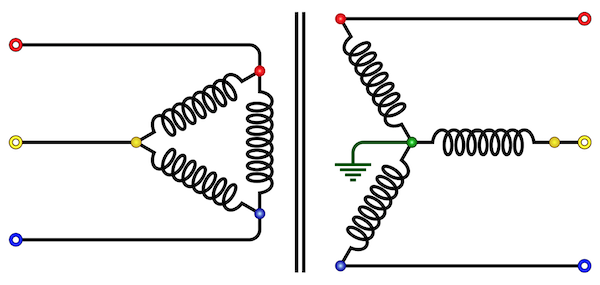
\includegraphics[width=400px]{triangulo-estrella-trafo.png}
        \end{center}
\end{enumerate}

Para la conexión estrella, tenemos que las tensiones de fase y línea primarias
siguen la relación
\begin{equation*}
  V_{L} = \sqrt{3} V_{F}
\end{equation*}
Y las intensidades
\begin{equation*}
  I_{L} = I_{F}
\end{equation*}

Para la conexión en triángulo , las tensiones de fase y línea son iguales
\begin{equation*}
  V_L = V_F
\end{equation*}
y las intensidades siguen la relación
\begin{equation*}
  I_L = \sqrt{3} I_F
\end{equation*}

En un transformador tenemos la relación de transformación
\begin{equation}
  R_t = \frac{I_{2L}}{I_{1L}} = \frac{V_{1L}}{V_{2L}} = \frac{N_1}{N_2}
\end{equation}

Para el ejemplo del triángulo-estrella ($\triangle Y$), podemos hallar las intensidades y
tensiones de fase y línea
\begin{equation*}
  \begin{split}
    I_{1L} = \sqrt{3} I_{1F}\\
    V_{1L} = V_{1F}
  \end{split}
\end{equation*}
Así, la relación de transformación nos da
\begin{equation*}
  I_{2L} = I_{1L} R_t \implies	I_{2L} = I_{1F} R_t \sqrt{3}
\end{equation*}
La tensión
\begin{equation*}
  V_{2L} = \frac{V_{1L}}{R_t} \implies V_{2F} = \frac{V_{1L}}{R_t \sqrt{3}}
\end{equation*}

Para un transformador triangulo-triangulo ($\triangle \triangle$) tenemos 
\begin{equation*}
  I_{2L} = I_{1L}R_t \implies I_{2F} = \frac{I_{1L} R_t}{\sqrt{3}} = \frac{I_{1F}R_t}{3}
\end{equation*}
Y la tensión 
\begin{equation*}
  V_{2L} = \frac{V_{1L}}{R_t} \implies V_{2F} = \frac{V_{1F}}{R_t} 
\end{equation*}


\end{document}
